\chapter{Explainability and Additional Experiments}
\section{Grad-AAM atom attribution}
The implementation targets the node activations produced by \texttt{model.drug\_encoder.transition3}, which have 228 channels per molecular atom before graph pooling and projection. For the scalar affinity prediction $s$, it differentiates the output with respect to these activations $A_{ic}$, where $i$ indexes atoms and $c$ indexes channels. It averages gradients over atom nodes to form channel weights, min--max normalizes those weights, then forms an atom score from the weighted activation channels and min--max normalizes the atom scores. In compact form:
\begin{align} g_c &= \frac{1}{N}\sum_{i=1}^{N}\frac{\partial s}{\partial A_{ic}},\qquad \alpha_c=\frac{g_c-\min_d g_d}{\max_d g_d-\min_d g_d+10^{-10}},\\ L_i &= \sum_c A_{ic}\alpha_c,\qquad \widetilde L_i=\frac{L_i-\min_j L_j}{\max_j L_j-\min_j L_j+10^{-10}}. \end{align}
The epsilon is the implementation's constant-range guard. No ReLU is applied to the atom score in this implementation. Values are mapped back to RDKit atom indices and rendered as a heat map. The interpretation is limited to model attribution for a selected input and checkpoint; highlighted atoms are not experimentally proven binding sites.

Five generated examples are in Figure~\ref{fig:grad-examples}; their true/predicted values and atom counts are in Table~\ref{tab:grad-values}. They come from the Davis test data selected by the visualization script. The images show relative atom scores and do not demonstrate protein-contact geometry.
\begin{figure}[H]\centering\begin{subfigure}{0.31\linewidth}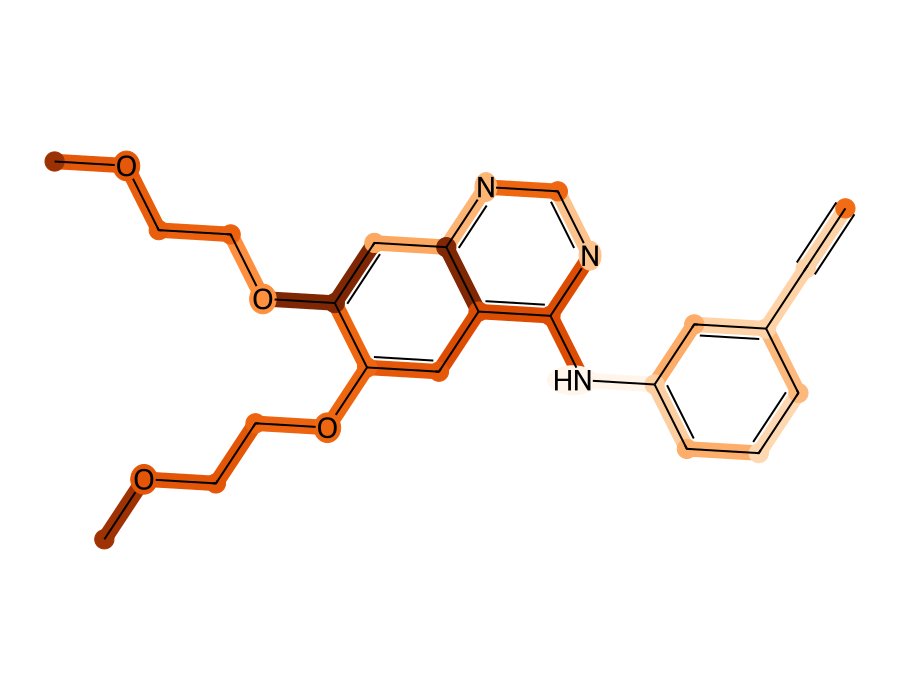
\includegraphics[width=\linewidth]{figures/grad_aam_0.png}\caption{Example 0}\end{subfigure}\begin{subfigure}{0.31\linewidth}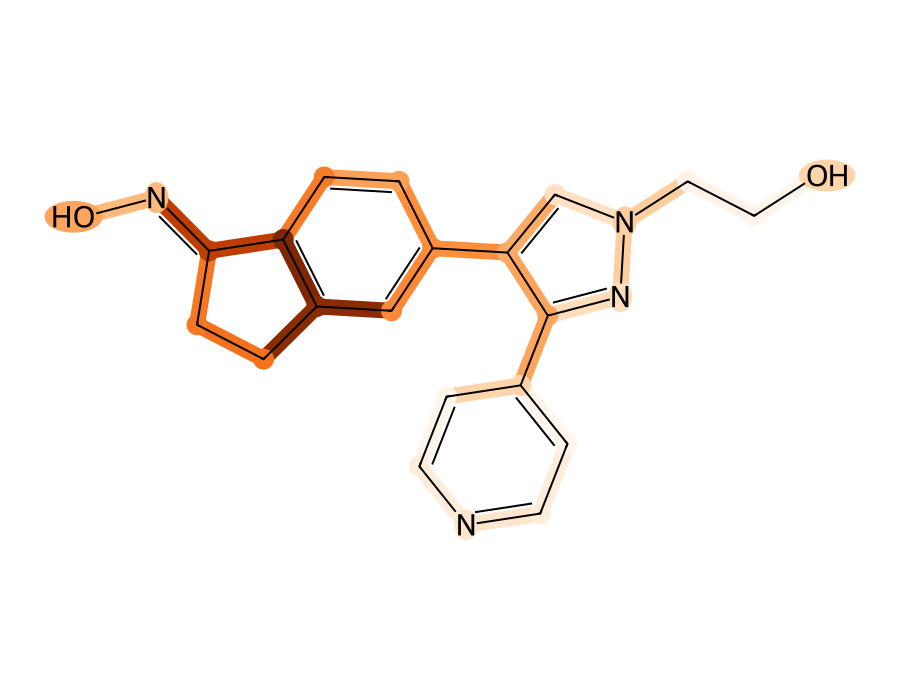
\includegraphics[width=\linewidth]{figures/grad_aam_1.png}\caption{Example 1}\end{subfigure}\begin{subfigure}{0.31\linewidth}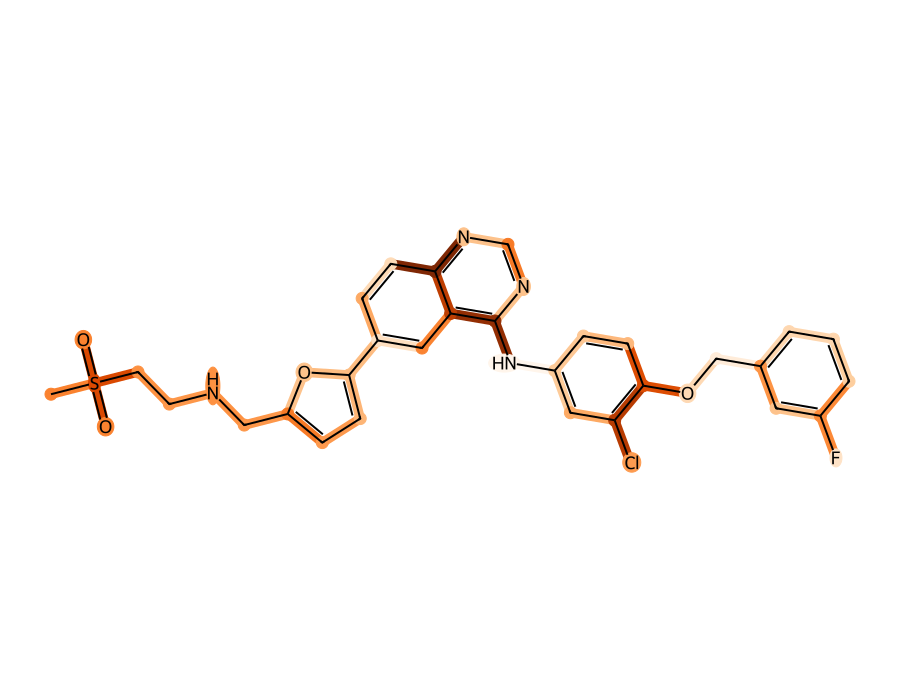
\includegraphics[width=\linewidth]{figures/grad_aam_2.png}\caption{Example 2}\end{subfigure}\\[4pt]\begin{subfigure}{0.31\linewidth}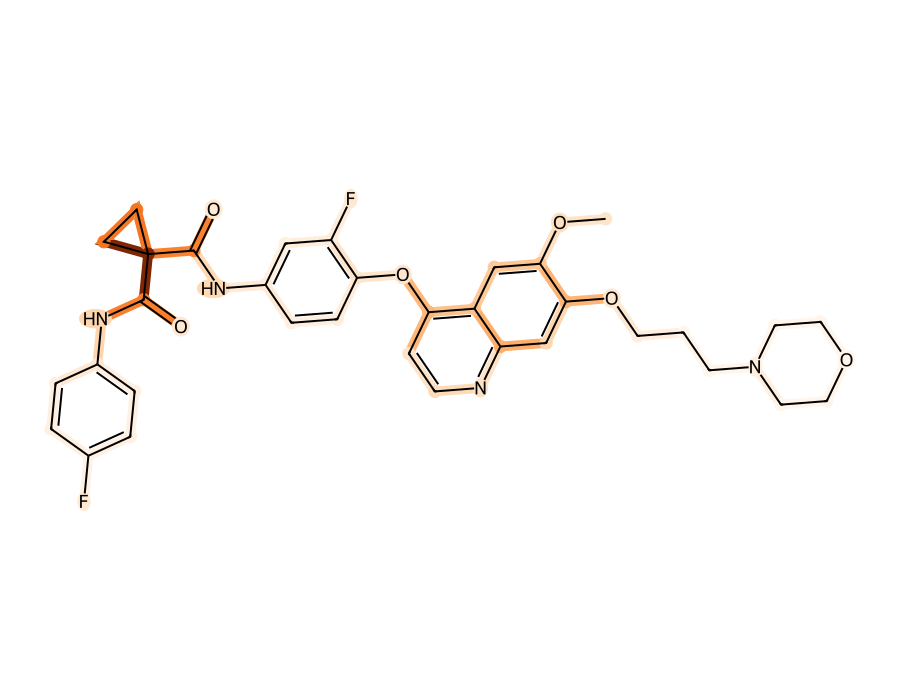
\includegraphics[width=\linewidth]{figures/grad_aam_3.png}\caption{Example 3}\end{subfigure}\begin{subfigure}{0.31\linewidth}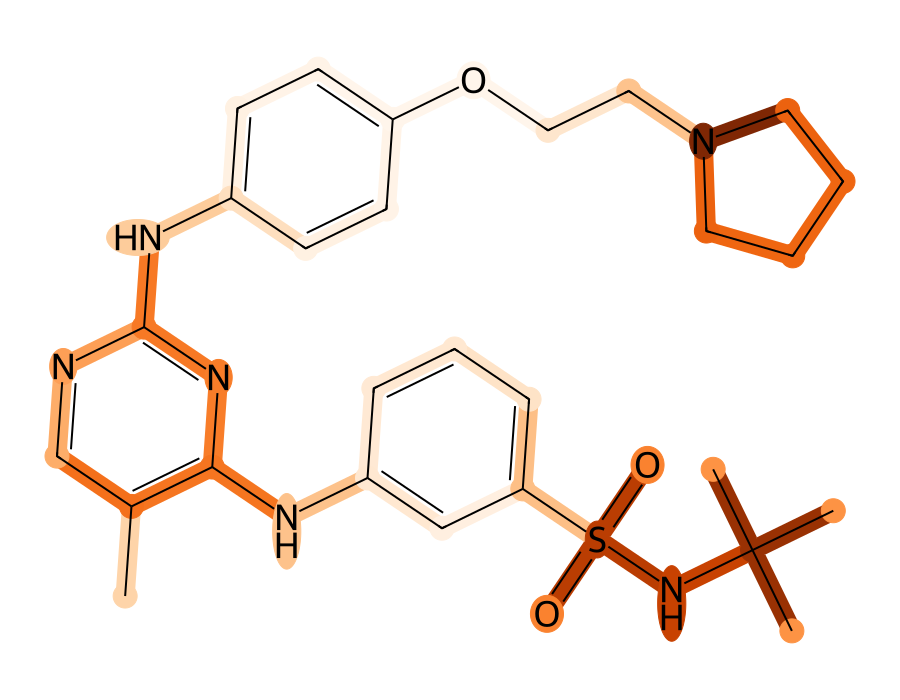
\includegraphics[width=\linewidth]{figures/grad_aam_4.png}\caption{Example 4}\end{subfigure}\caption{Five stored Grad-AAM atom-attribution outputs. Heat-map intensities are model-derived relative importance values.}\label{fig:grad-examples}\end{figure}
\begin{table}[H]\centering\small\caption{Metadata for the five Grad-AAM examples}\label{tab:grad-values}\begin{tabular}{rrrrr}\toprule Index & True affinity & Predicted & Absolute error & Atoms\\\midrule 0 & 5.000000 & 5.552389 & 0.552389 & 29\\1 & 5.000000 & 5.258000 & 0.258000 & 25\\2 & 5.000000 & 5.100961 & 0.100961 & 40\\3 & 8.823909 & 8.305184 & 0.518724 & 46\\4 & 5.000000 & 5.434842 & 0.434842 & 37\\\bottomrule\end{tabular}\end{table}

\section{Sequence-adjacency 2D Protein-GNN experiment}
An additional standalone experiment represents each unique target sequence as a graph: residues are nodes, the 20 standard amino acids use one-hot features, and consecutive residues are connected in both directions. Thus an $L$-residue sequence has $L$ nodes and $2(L-1)$ directed edges. It contains residue identity and sequence adjacency only; it has no measured 3D coordinates, spatial contacts, or tertiary-structure edges. The encoder uses GCNConv $20\to64$, ReLU, GCNConv $64\to96$, ReLU, and global mean pooling. The protein vector is concatenated with the existing 96-D MGNN drug representation and passed to the same 192-dimensional-input MLP.

\begin{table}[H]\centering\caption{Standalone 2D Protein-GNN independent test metrics}\label{tab:proteingnn}\begin{tabular}{lr}\toprule Metric & Value\\\midrule MSE & 0.6517305271\\RMSE & 0.8072982888\\CI & 0.7596736960\\$r_m^2$ & 0.2090044869\\Best validation epoch / MSE & 29 / 0.5732540258\\\bottomrule\end{tabular}\end{table}
This experiment asks whether a graph encoder over sequence-neighbor residues is a viable alternative to the main MCNN representation within the recorded prototype. It is an observed run only; it does not establish a general claim about protein GNNs. Sequence adjacency alone may miss spatially adjacent residues that are distant in primary sequence and cannot encode a folded binding pocket. Figure~\ref{fig:compare} shows the saved training comparison. The main and comparison experiment differ in their trained protein encoders but share the listed Davis fold and nominal seed/configuration; the comparison figure is descriptive, not a controlled repeated study.
\begin{figure}[H]\centering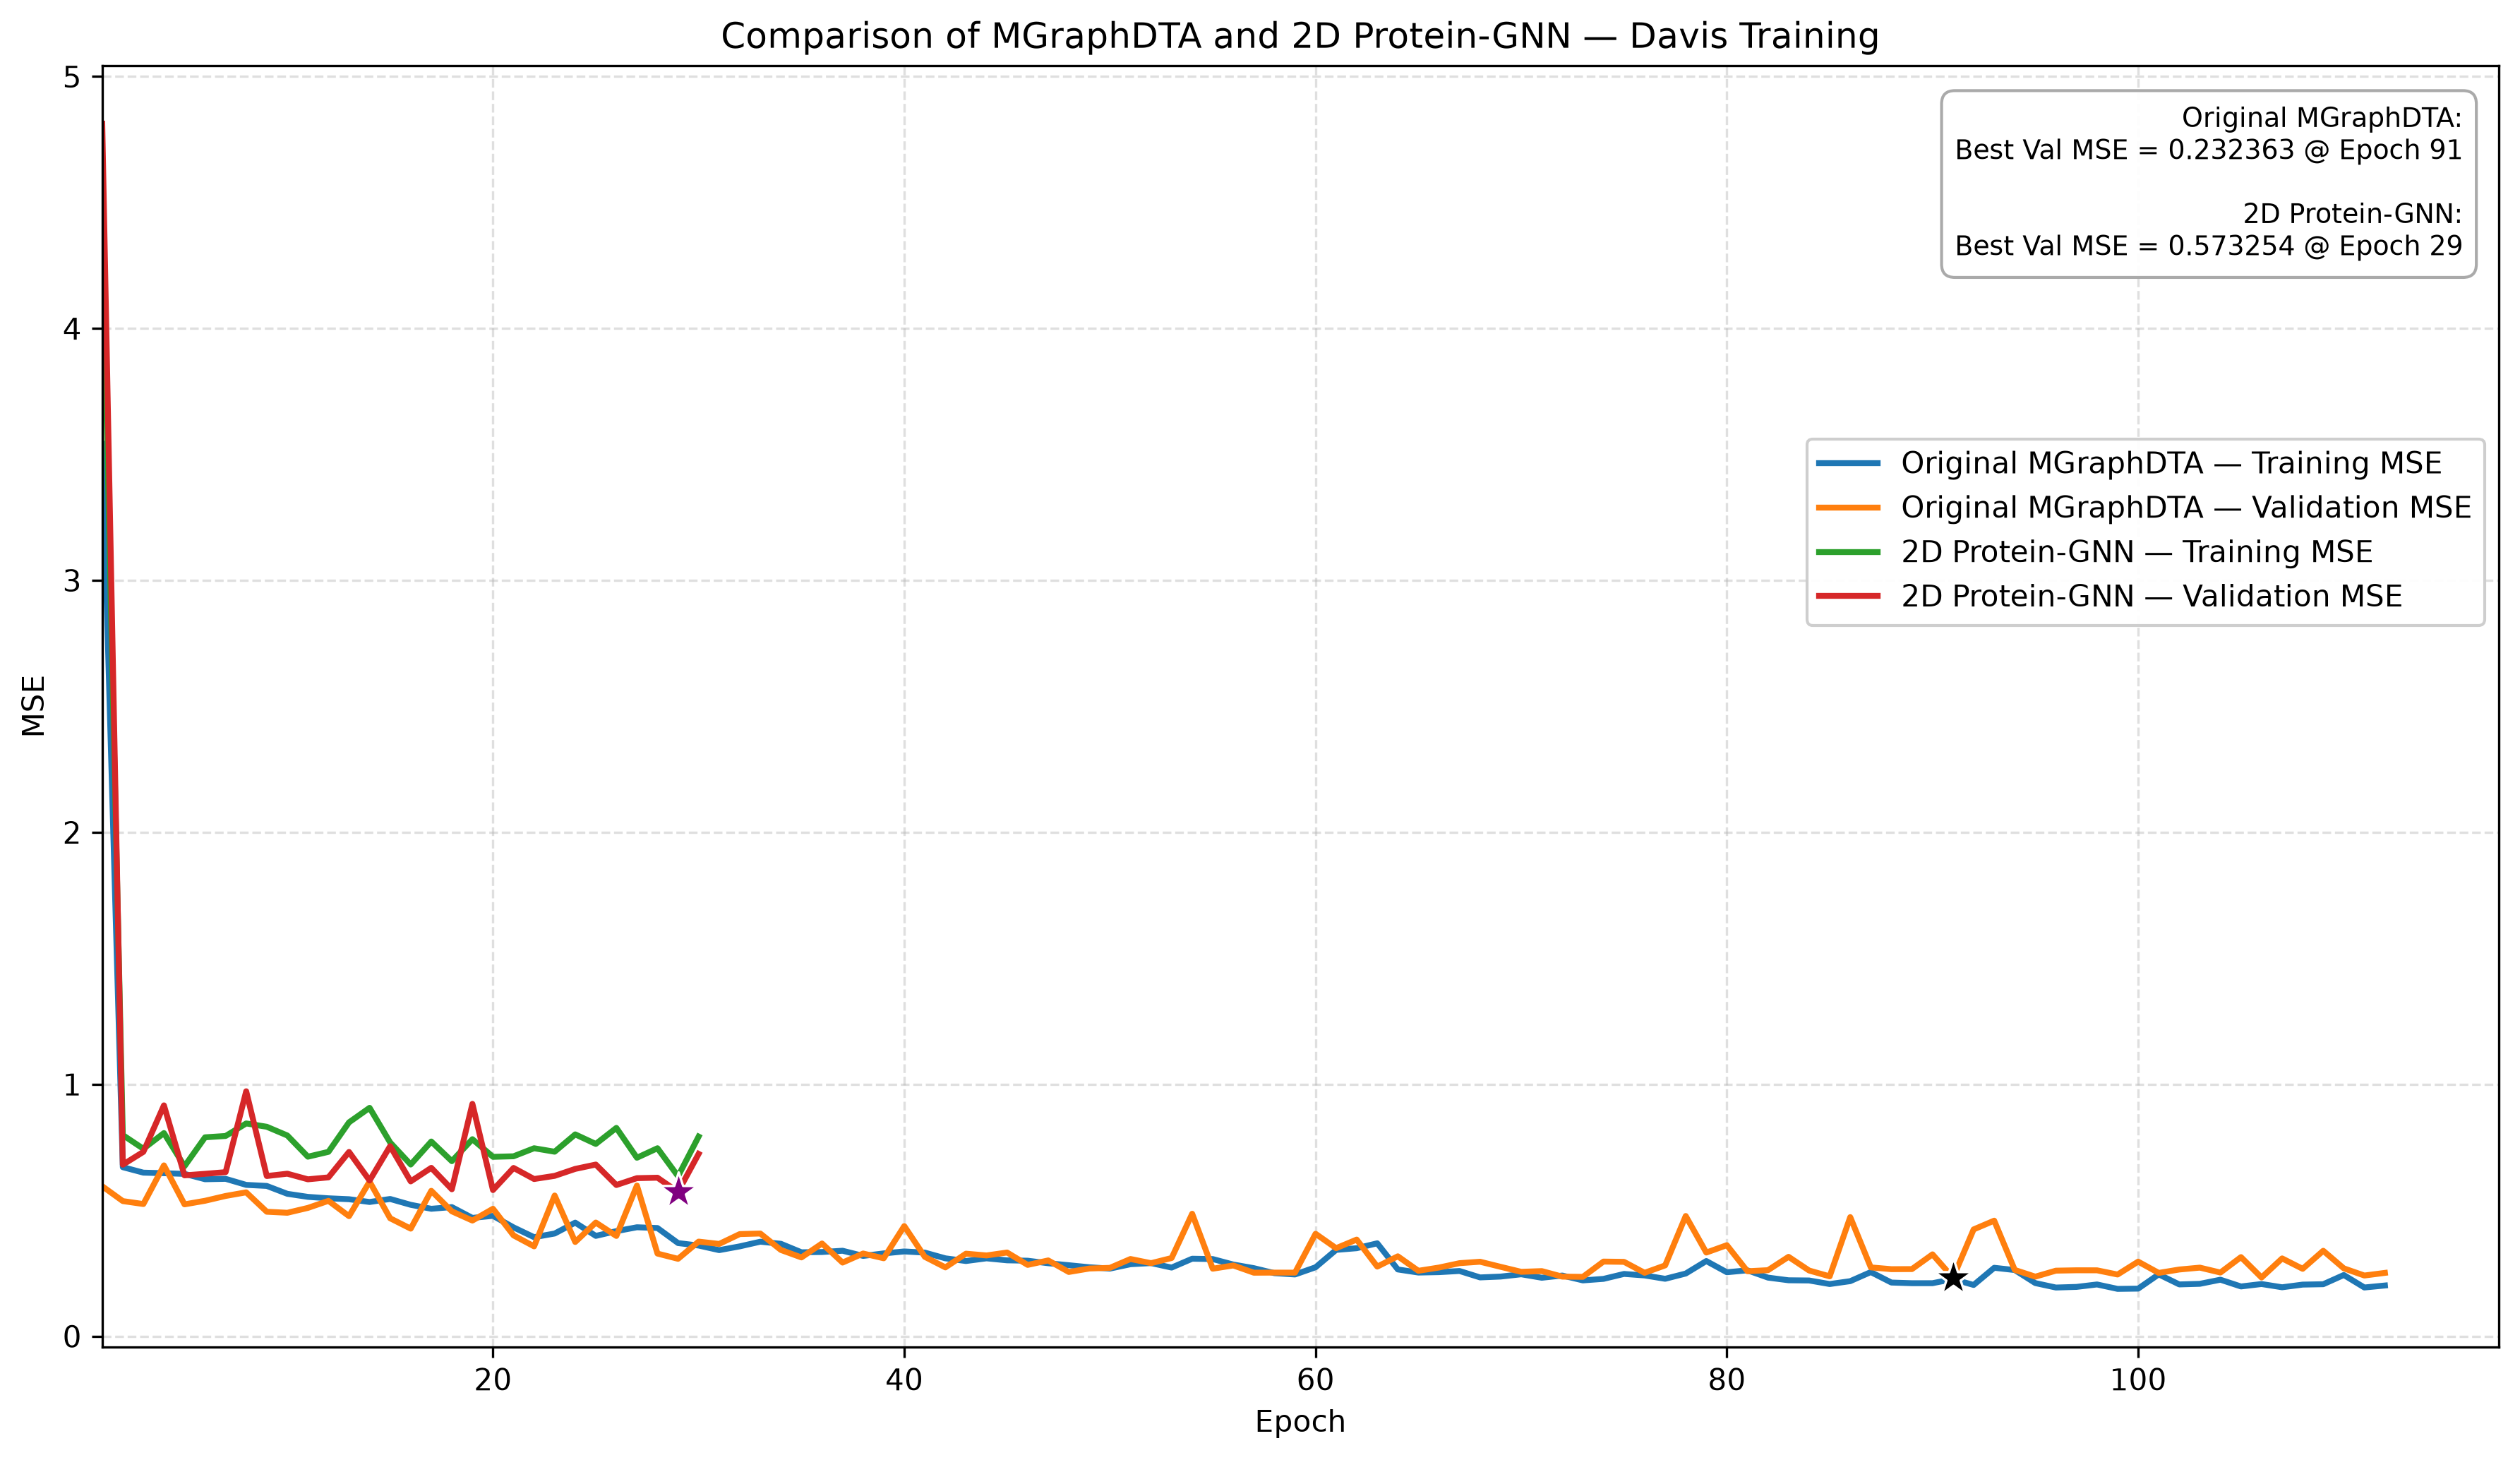
\includegraphics[width=0.9\linewidth]{figures/training_comparison.png}\caption{Generated MGraphDTA versus 2D Protein-GNN training/validation history comparison.}\label{fig:compare}\end{figure}
The project generated 379 unique sequence graphs representing 442 target IDs. Across the graphs there are 282,298 residue nodes and 563,838 directed edges; sequence lengths range from 244 to 2,549 residues (mean 744.85), and two residues have non-standard/unknown identities. Each standard residue uses a 20-dimensional one-hot feature; unknown rows are all-zero. For AKT1, the graph has 480 residues/nodes and 958 directed edges. The graph is a sequence-adjacency graph, not a 3D structure.
\begin{table}[H]\centering\small\caption{Verified sequence-adjacency protein graph construction summary}\label{tab:protein-graphs}\begin{tabular}{lr}\toprule Quantity & Value\\\midrule Unique sequence graphs & 379\\Davis target IDs represented & 442\\Total residue nodes & 282,298\\Total directed edges & 563,838\\Sequence length, minimum / maximum & 244 / 2,549\\Mean sequence length & 744.85\\Unknown/non-standard residues & 2\\Node features & 20-D one-hot\\AKT1 residues/nodes & 480\\AKT1 directed edges & 958\\\bottomrule\end{tabular}\end{table}
The AKT1 molecular-style visualization displays only the first 50 residues for readability; it does not change the stored 480-node graph.
\begin{figure}[H]\centering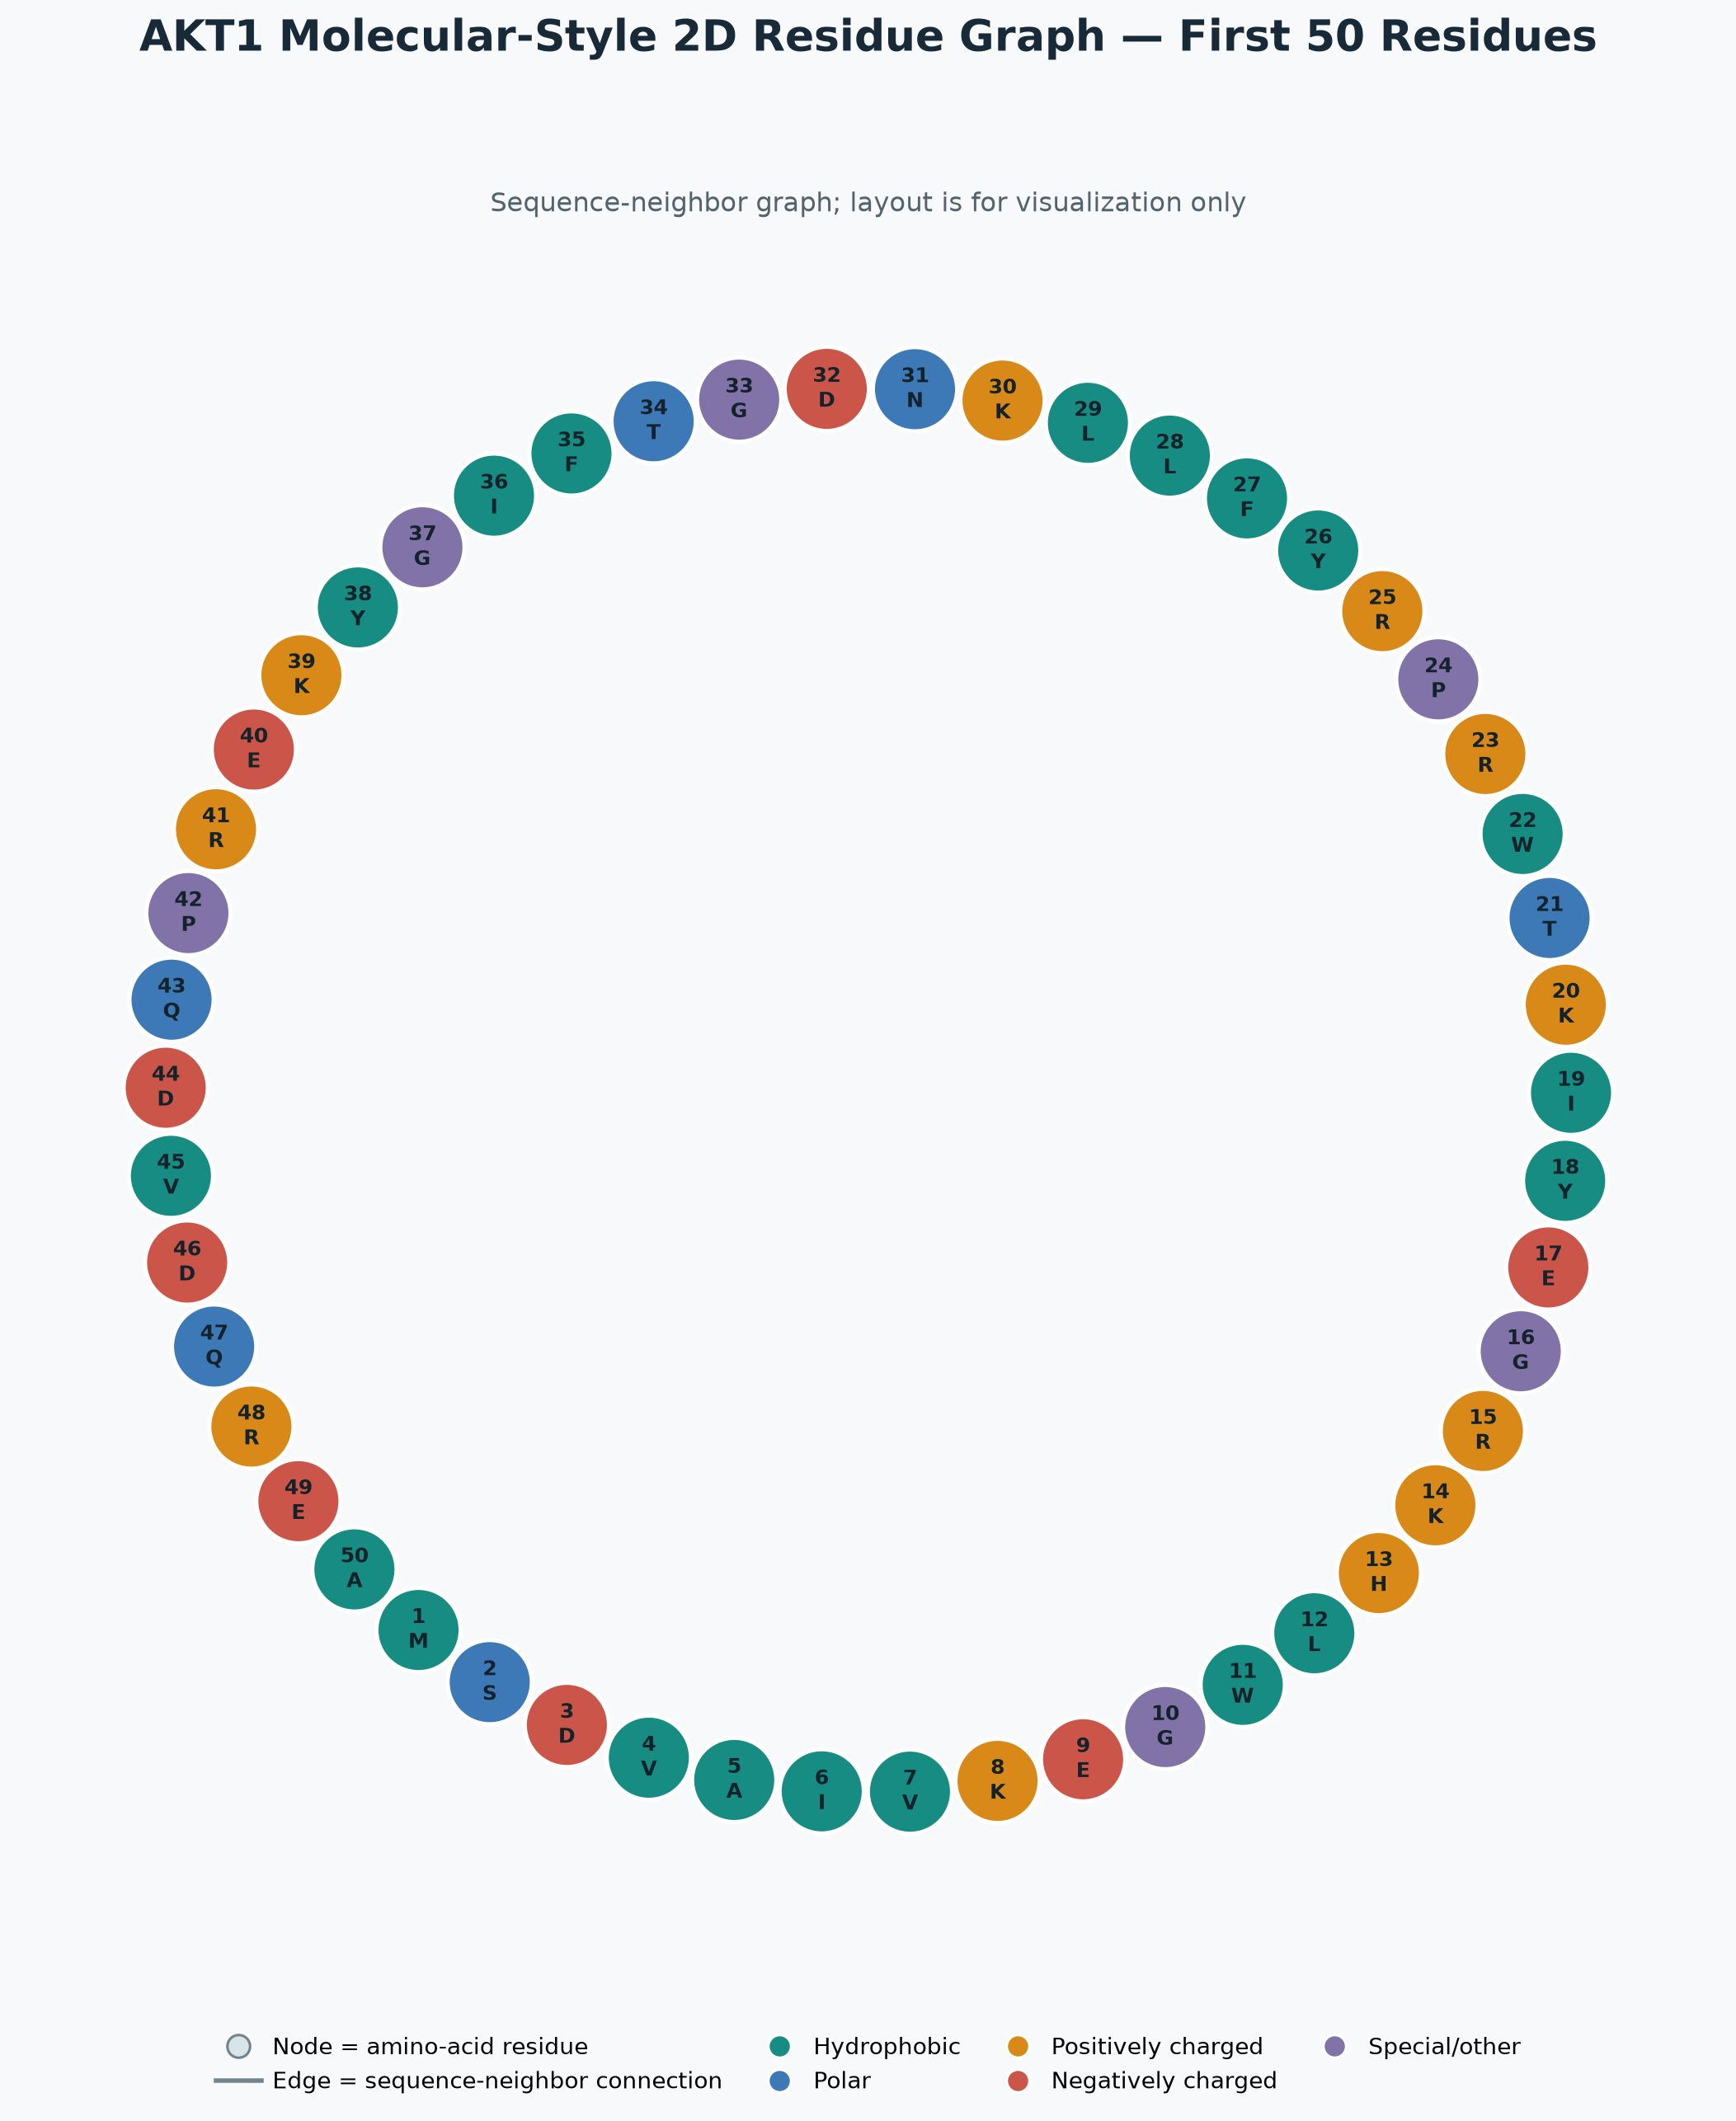
\includegraphics[width=0.85\linewidth]{figures/akt1_graph.png}\caption{AKT1 sequence-adjacency graph visualization showing the first 50 of 480 residue nodes. Edges encode consecutive sequence positions, not spatial contacts.}\label{fig:akt1}\end{figure}

\section{Preliminary protein structure audit}
The repository contains the AKT1 inspection script and a detailed FLT4 sample audit, but no saved aggregate RCSB audit CSV/JSON was found. Table~\ref{tab:rcsb-audit} records the project-supplied aggregate summary. These counts are transcribed as project-reported values; the absent aggregate output means they could not be independently recomputed from repository artifacts. The audit is preliminary and incomplete. The counts must not be converted into or described as a definitive structure-coverage percentage; no audit-wide coverage percentage is reported here.

\begin{table}[H]\centering\small\caption{Project-reported preliminary RCSB audit summary; aggregate source file unavailable for independent verification}\label{tab:rcsb-audit}\begin{tabular}{lr}\toprule Audit measure & Count\\\midrule Unique protein sequences searched & 379\\Full matches & 87\\Partial matches & 211\\No reliable match & 15\\Query errors & 66\\Successfully processed sequence searches & 313 / 379\\Target IDs with a structure match under the criteria & 360 / 442\\\bottomrule\end{tabular}\end{table}

The reported match criteria are: experimental structure; sequence identity at least 90\%; at least 100 aligned/matched residues; a full match requires at least 90\% sequence coverage; otherwise an accepted match is partial. Counts should be read under those criteria, not as proof of a complete experimentally resolved proteome.

One documented example concerns Davis sample 3, the FLT4 target with Foretinib. The local verification note reports partial FLT4 extracellular-domain records (4BSJ and 4BSK) but no verified experimental complex containing Foretinib bound to the Davis FLT4 kinase site. It identifies Foretinib-containing structures for other proteins, which do not establish an FLT4 complex. The repository script \texttt{scripts/inspect\_akt1\_structure.py} defines sequence alignment for the AKT1 chain in 9AAA and checks for atom-site versus IHM sphere-site records. The project-reported outcome is that the sequence matched, while the entry used an integrative-hybrid/coarse-grained representation without standard atom-coordinate records; it was therefore not treated as a conventional atomic structure. The script is available, but its run output/inspection CSV is absent, so the specific sequence-match values and record classification could not be independently rechecked. No definitive structure-coverage claim is made.

\section{Separate experimental structure demonstrations}
The five structure examples below are educational demonstrations based on deposited coordinate structures and locally generated interaction CSVs/diagrams. They are not Davis training samples, are not predictions from MGraphDTA, and are not Grad-AAM explanations. The CSVs count geometrically detected interactions under the scripts' criteria; values should be understood as computed contacts on the deposited structures.
\begin{table}[H]\centering\small\caption{Independent structural demonstration set}\label{tab:structures}\begin{tabular}{llllrr}\toprule PDB & Protein & Ligand & Method & Resolution (\AA) & Contacts\\\midrule 2HYY & ABL1 kinase & Imatinib (STI571) & X-ray & 2.40 & 18\\2ITZ & EGFR L858R kinase & Gefitinib & X-ray & 2.80 & 9\\1M17 & EGFR kinase & Erlotinib & X-ray & 2.60 & 6\\1HSG & HIV-1 protease & L-735,524 (indinavir) & X-ray & 2.00 & 23\\1STP & Streptavidin & Biotin & X-ray & 2.60 & 8\\\bottomrule\end{tabular}\end{table}
The generated CSVs include hydrogen bonds and hydrophobic contacts where detected, as well as selected interaction types such as aromatic and cation--pi contacts or halogen bonding. For example, the 2HYY output includes hydrophobic, pi--pi, and pi--cation contacts; 2ITZ includes a hydrogen bond, hydrophobic contacts, pi--cation and a halogen bond; 1M17 includes a hydrogen bond and hydrophobic contacts; 1HSG includes polar hydrogen-bond contacts and hydrophobic contacts; and the 1STP table includes polar and nonpolar contacts. Exact geometries and atom labels are preserved in each corresponding CSV. These are geometric analyses of experimental coordinates, not model predictions.
\begin{figure}[H]\centering\begin{subfigure}{0.48\linewidth}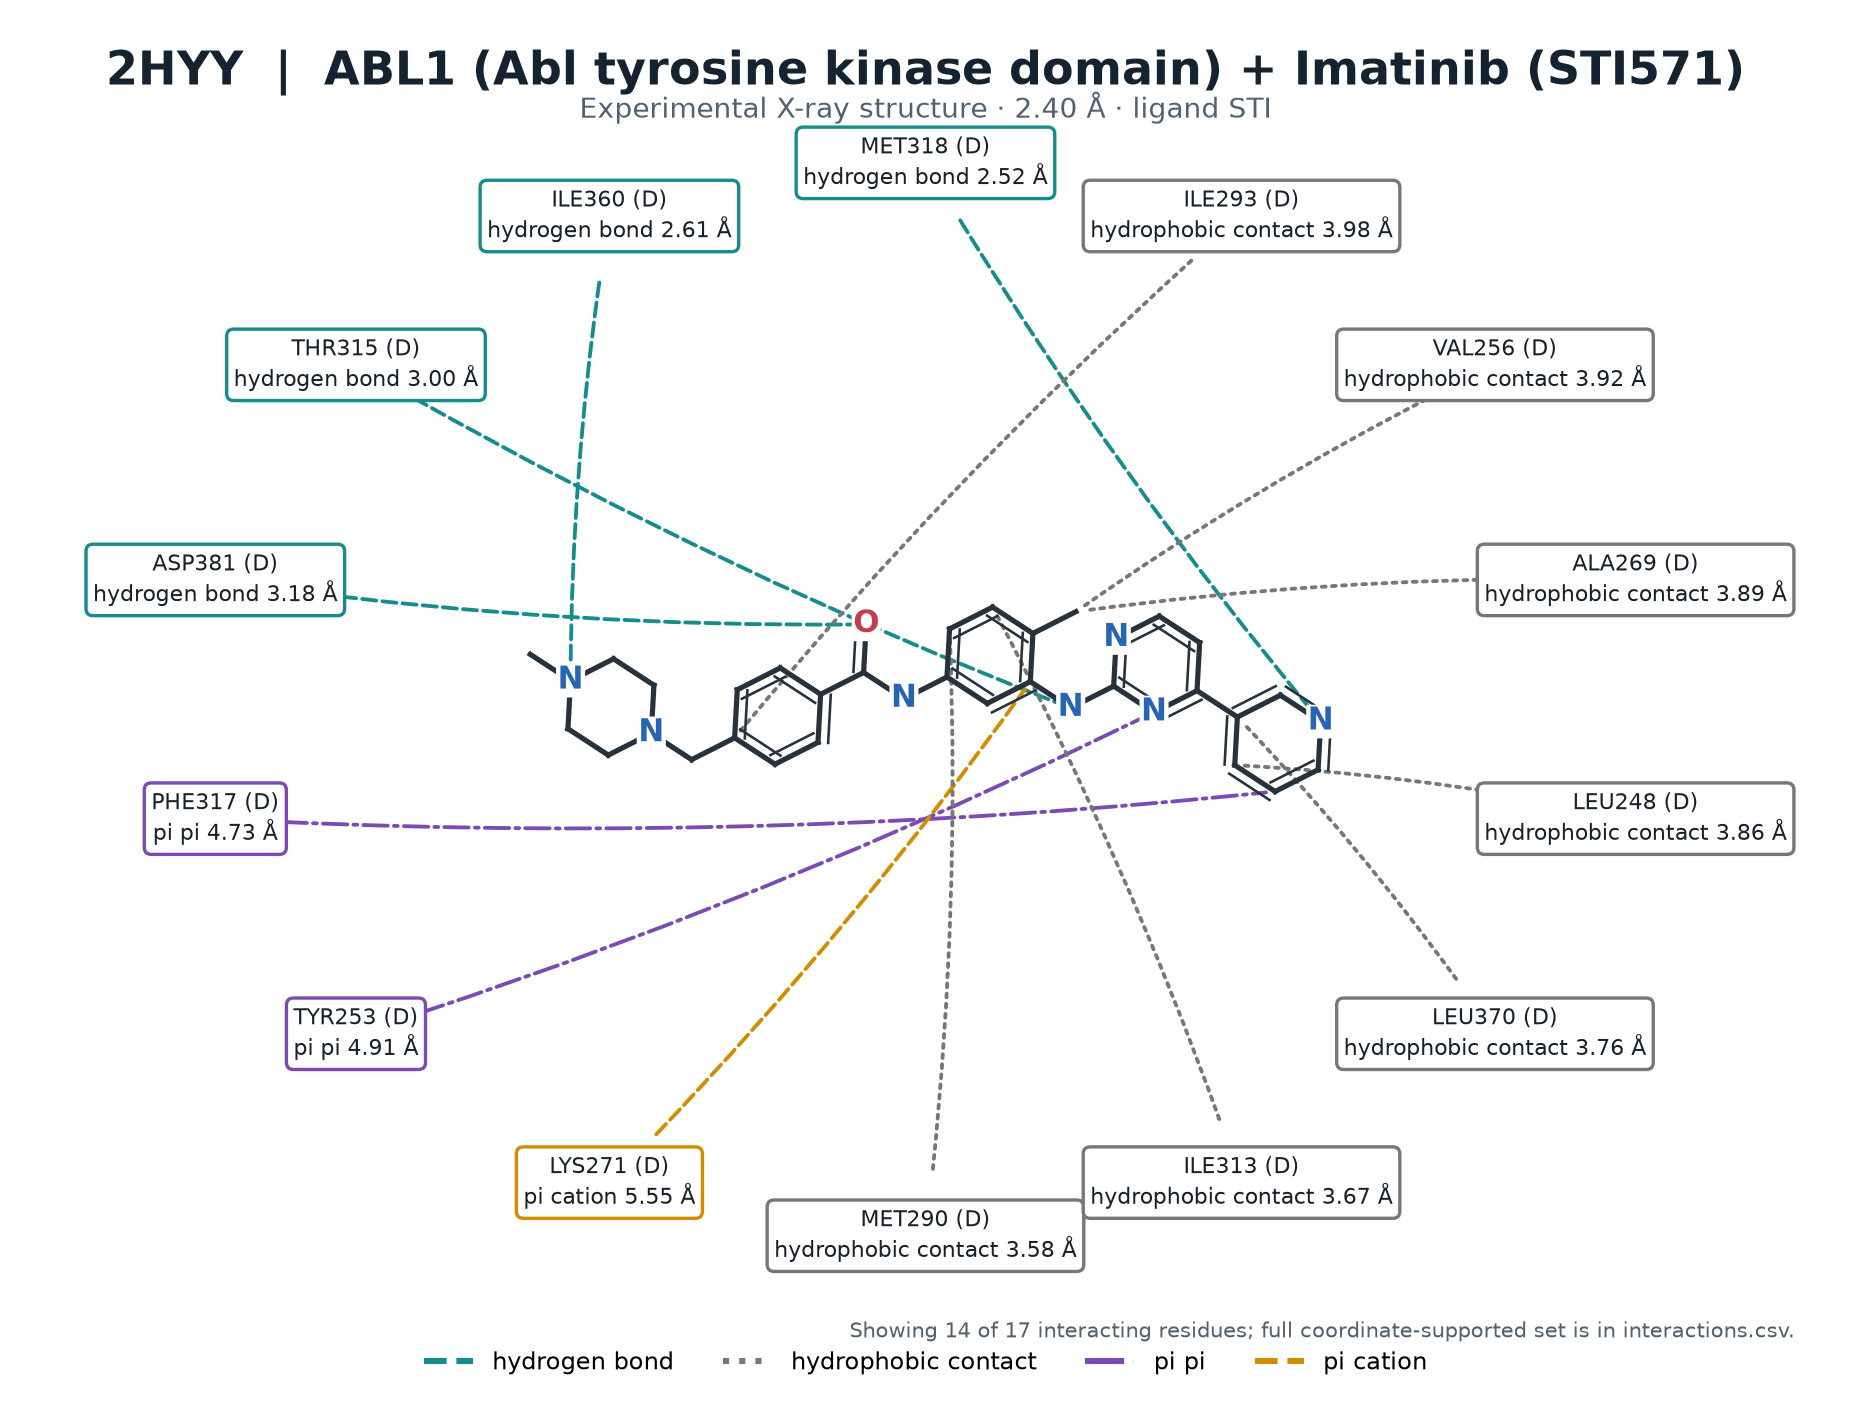
\includegraphics[width=\linewidth]{figures/interaction_2HYY.png}\caption{2HYY: ABL1--imatinib}\end{subfigure}\begin{subfigure}{0.48\linewidth}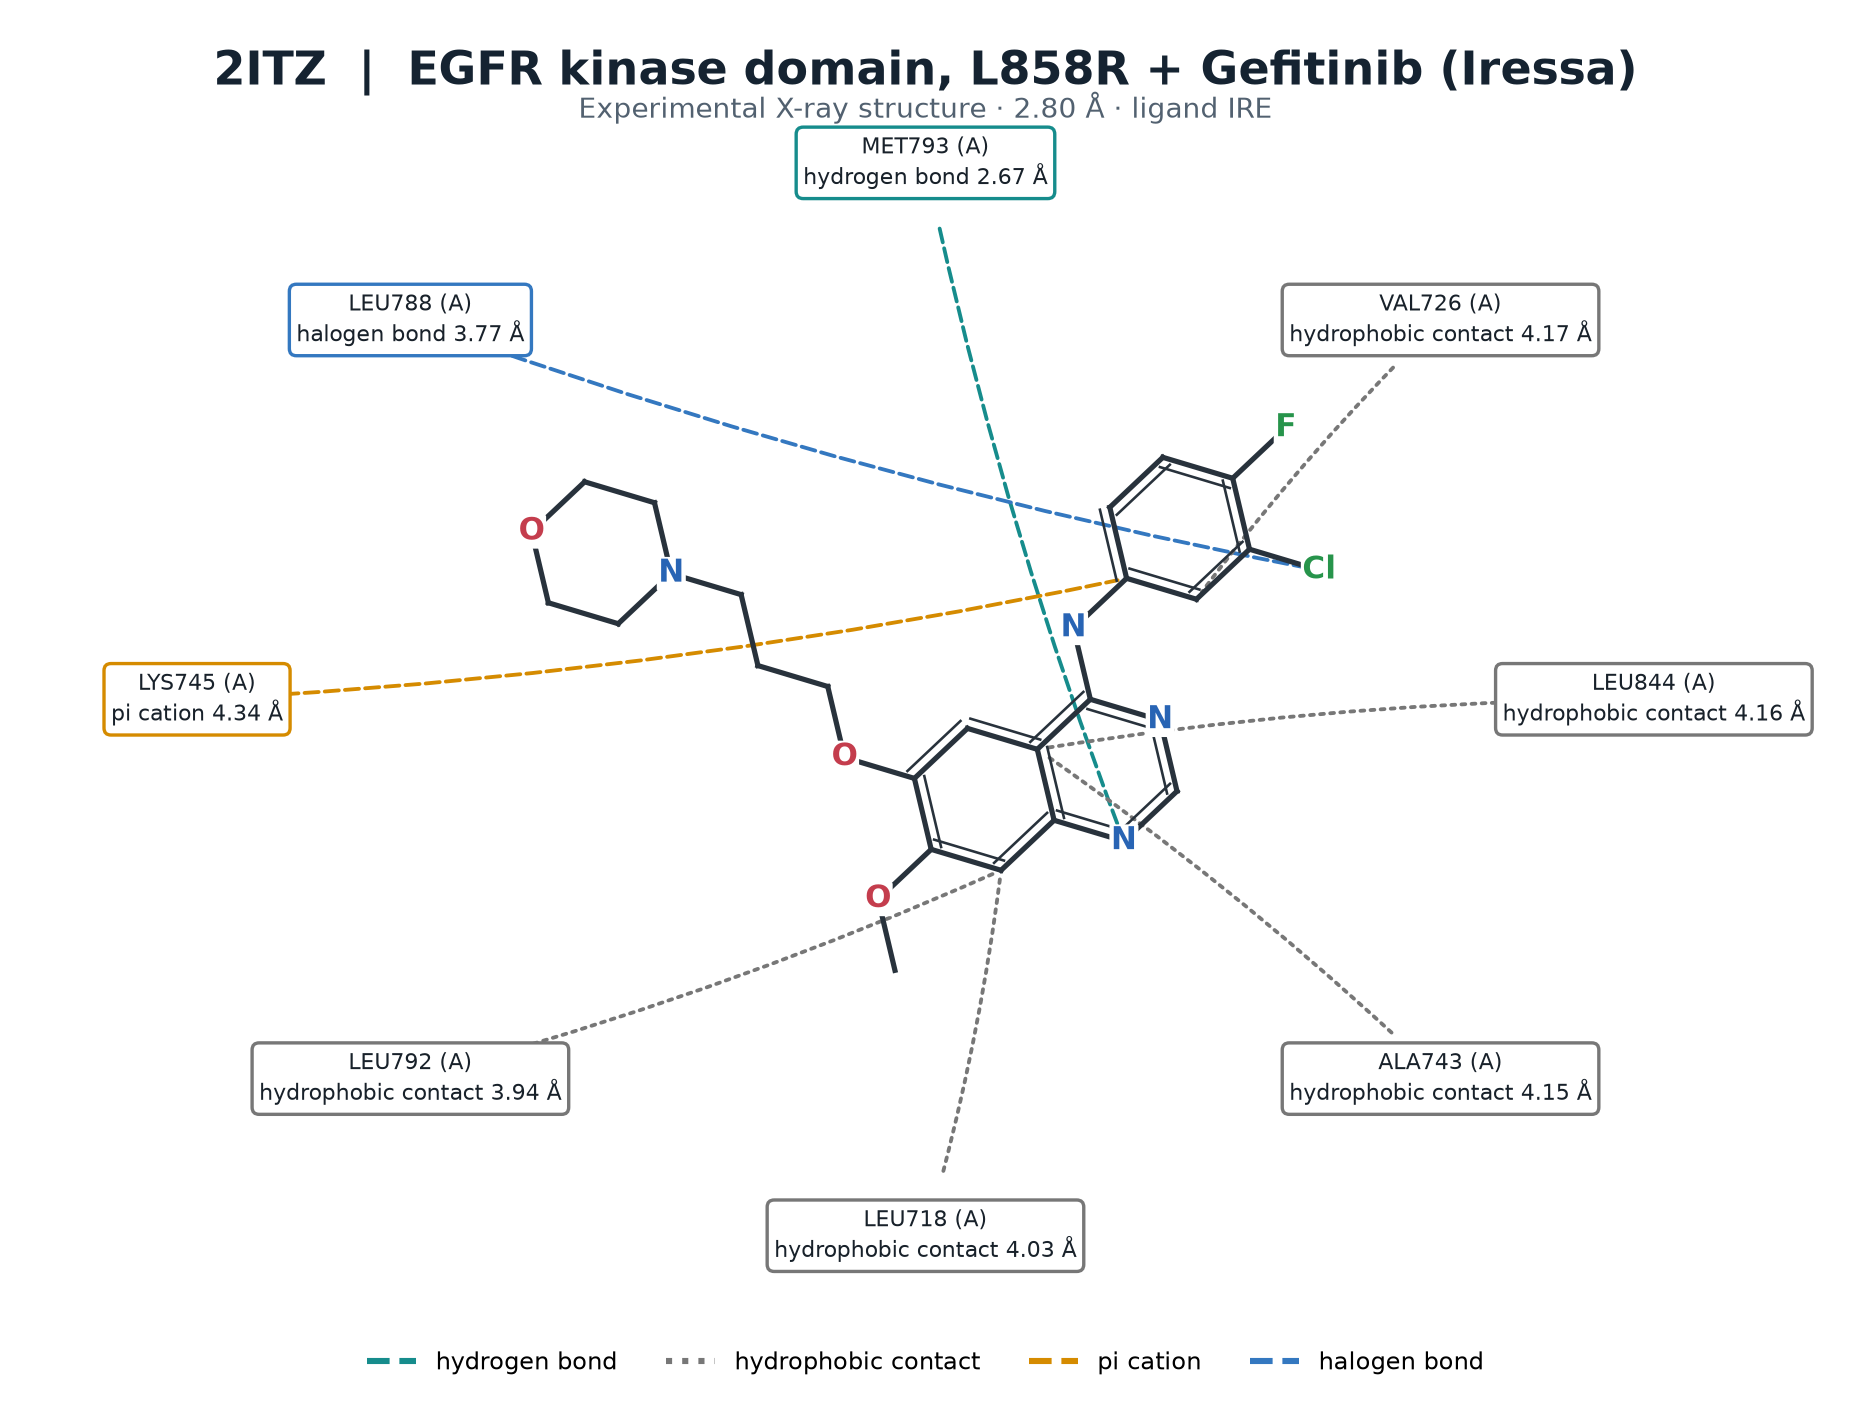
\includegraphics[width=\linewidth]{figures/interaction_2ITZ.png}\caption{2ITZ: EGFR L858R--gefitinib}\end{subfigure}\\\begin{subfigure}{0.48\linewidth}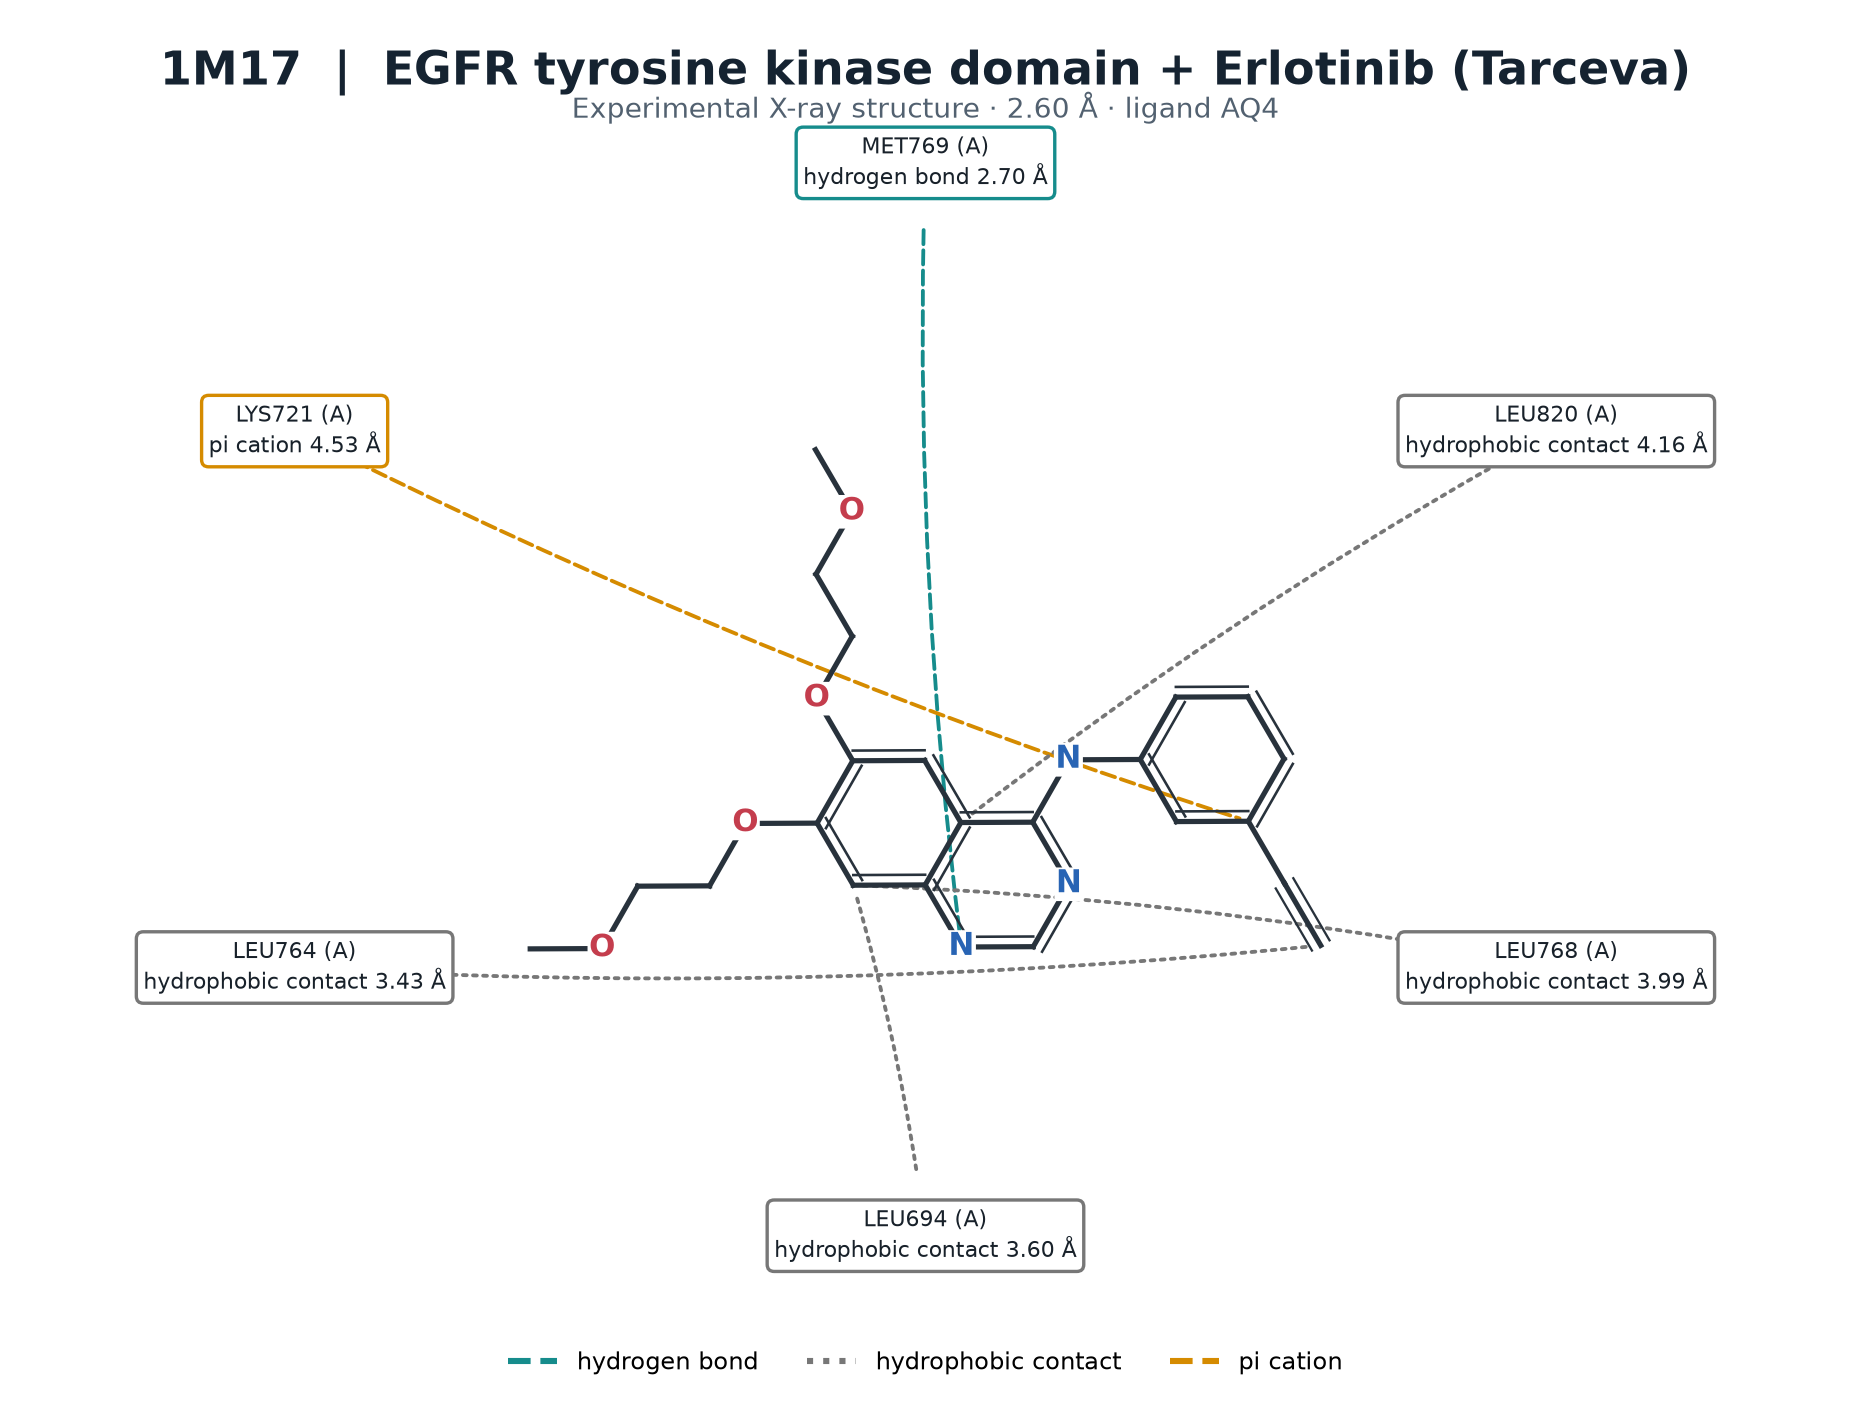
\includegraphics[width=\linewidth]{figures/interaction_1M17.png}\caption{1M17: EGFR--erlotinib}\end{subfigure}\begin{subfigure}{0.48\linewidth}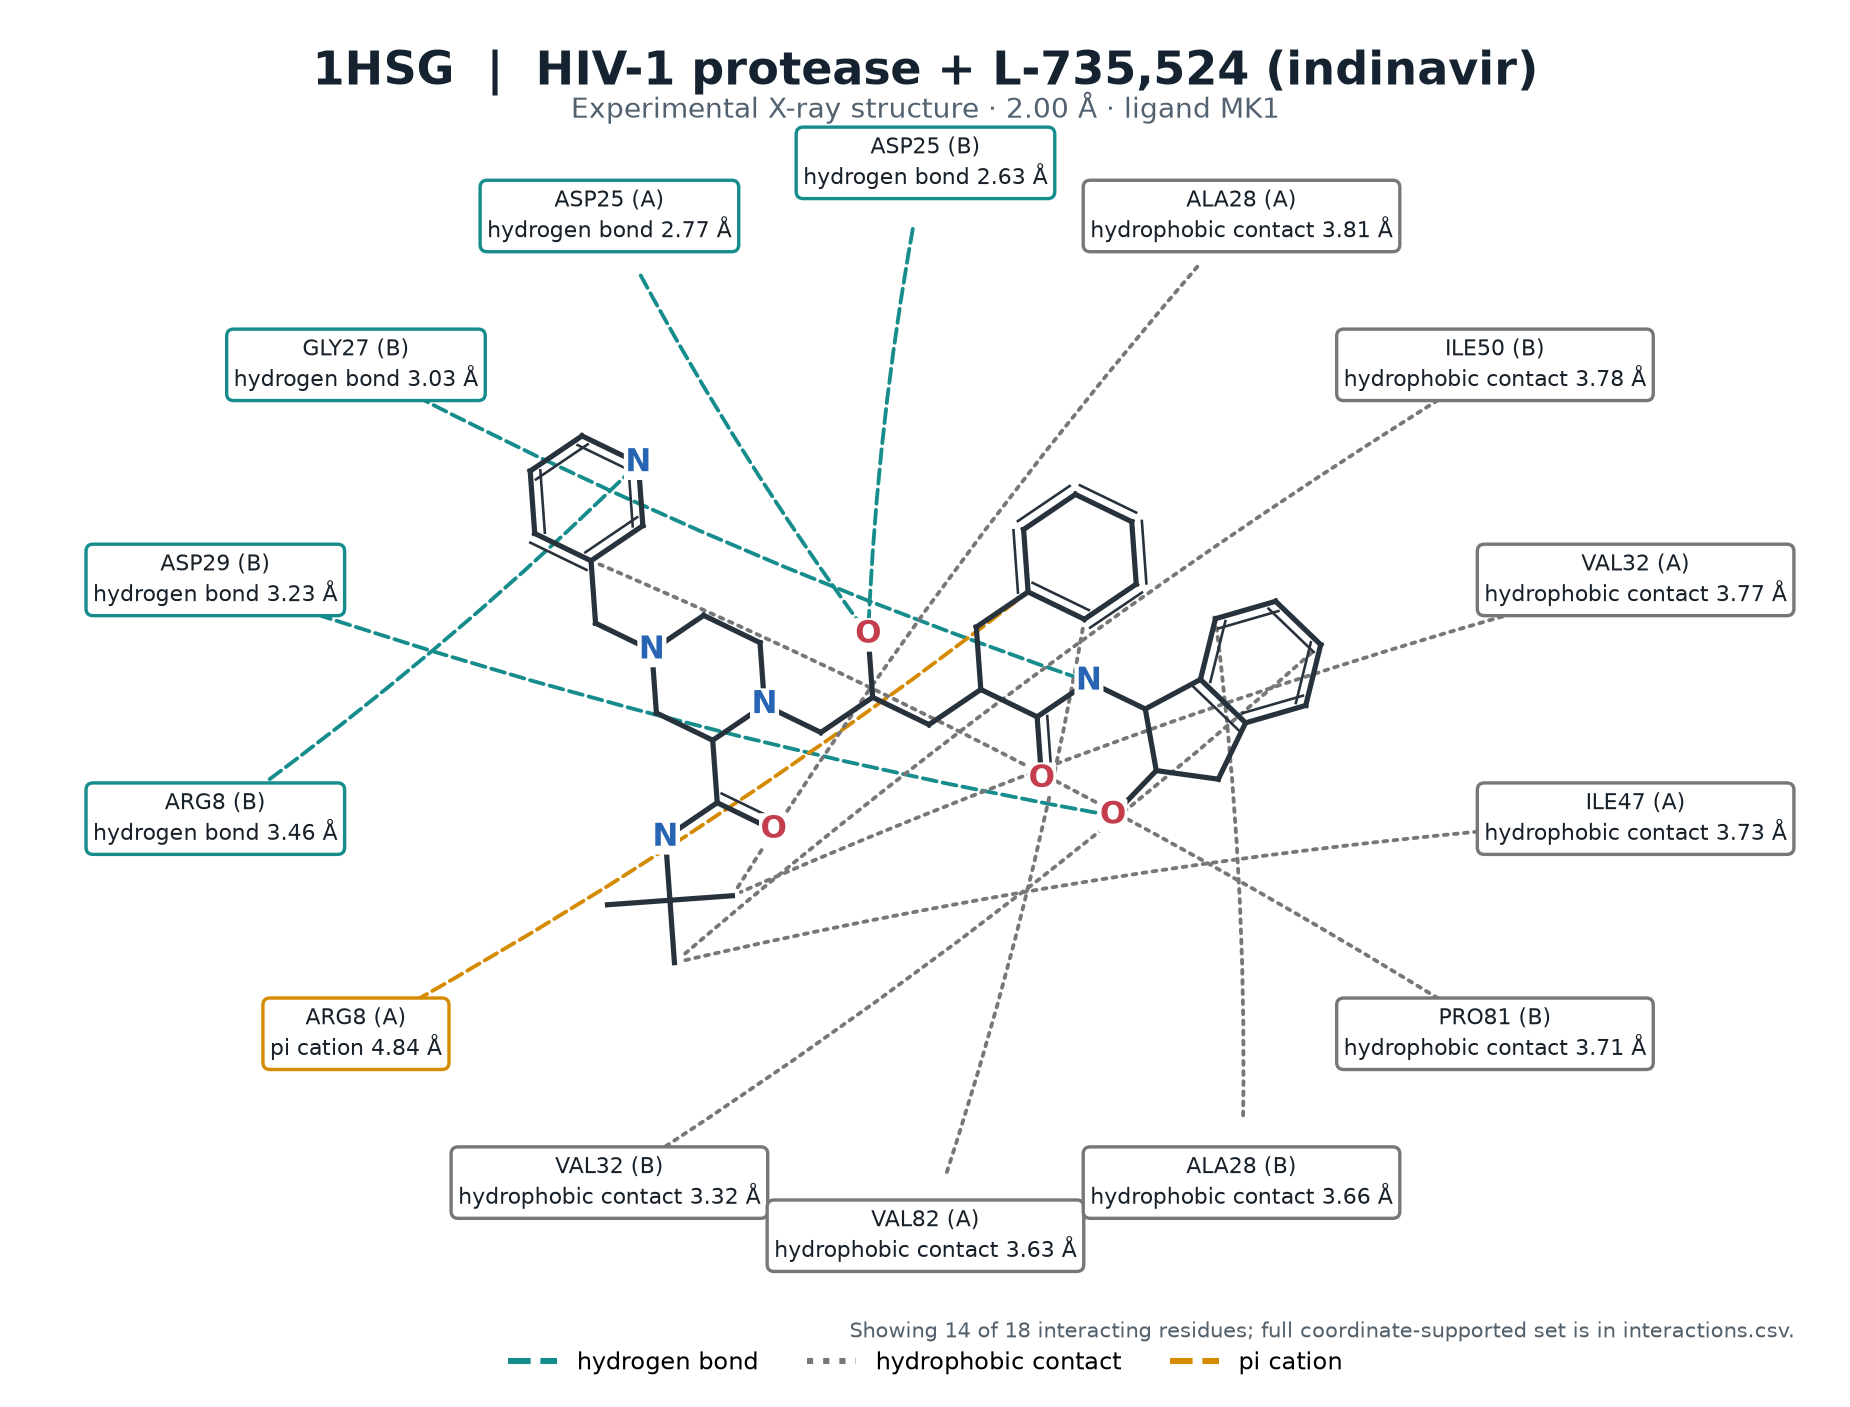
\includegraphics[width=\linewidth]{figures/interaction_1HSG.png}\caption{1HSG: HIV-1 protease--indinavir}\end{subfigure}\\\begin{subfigure}{0.55\linewidth}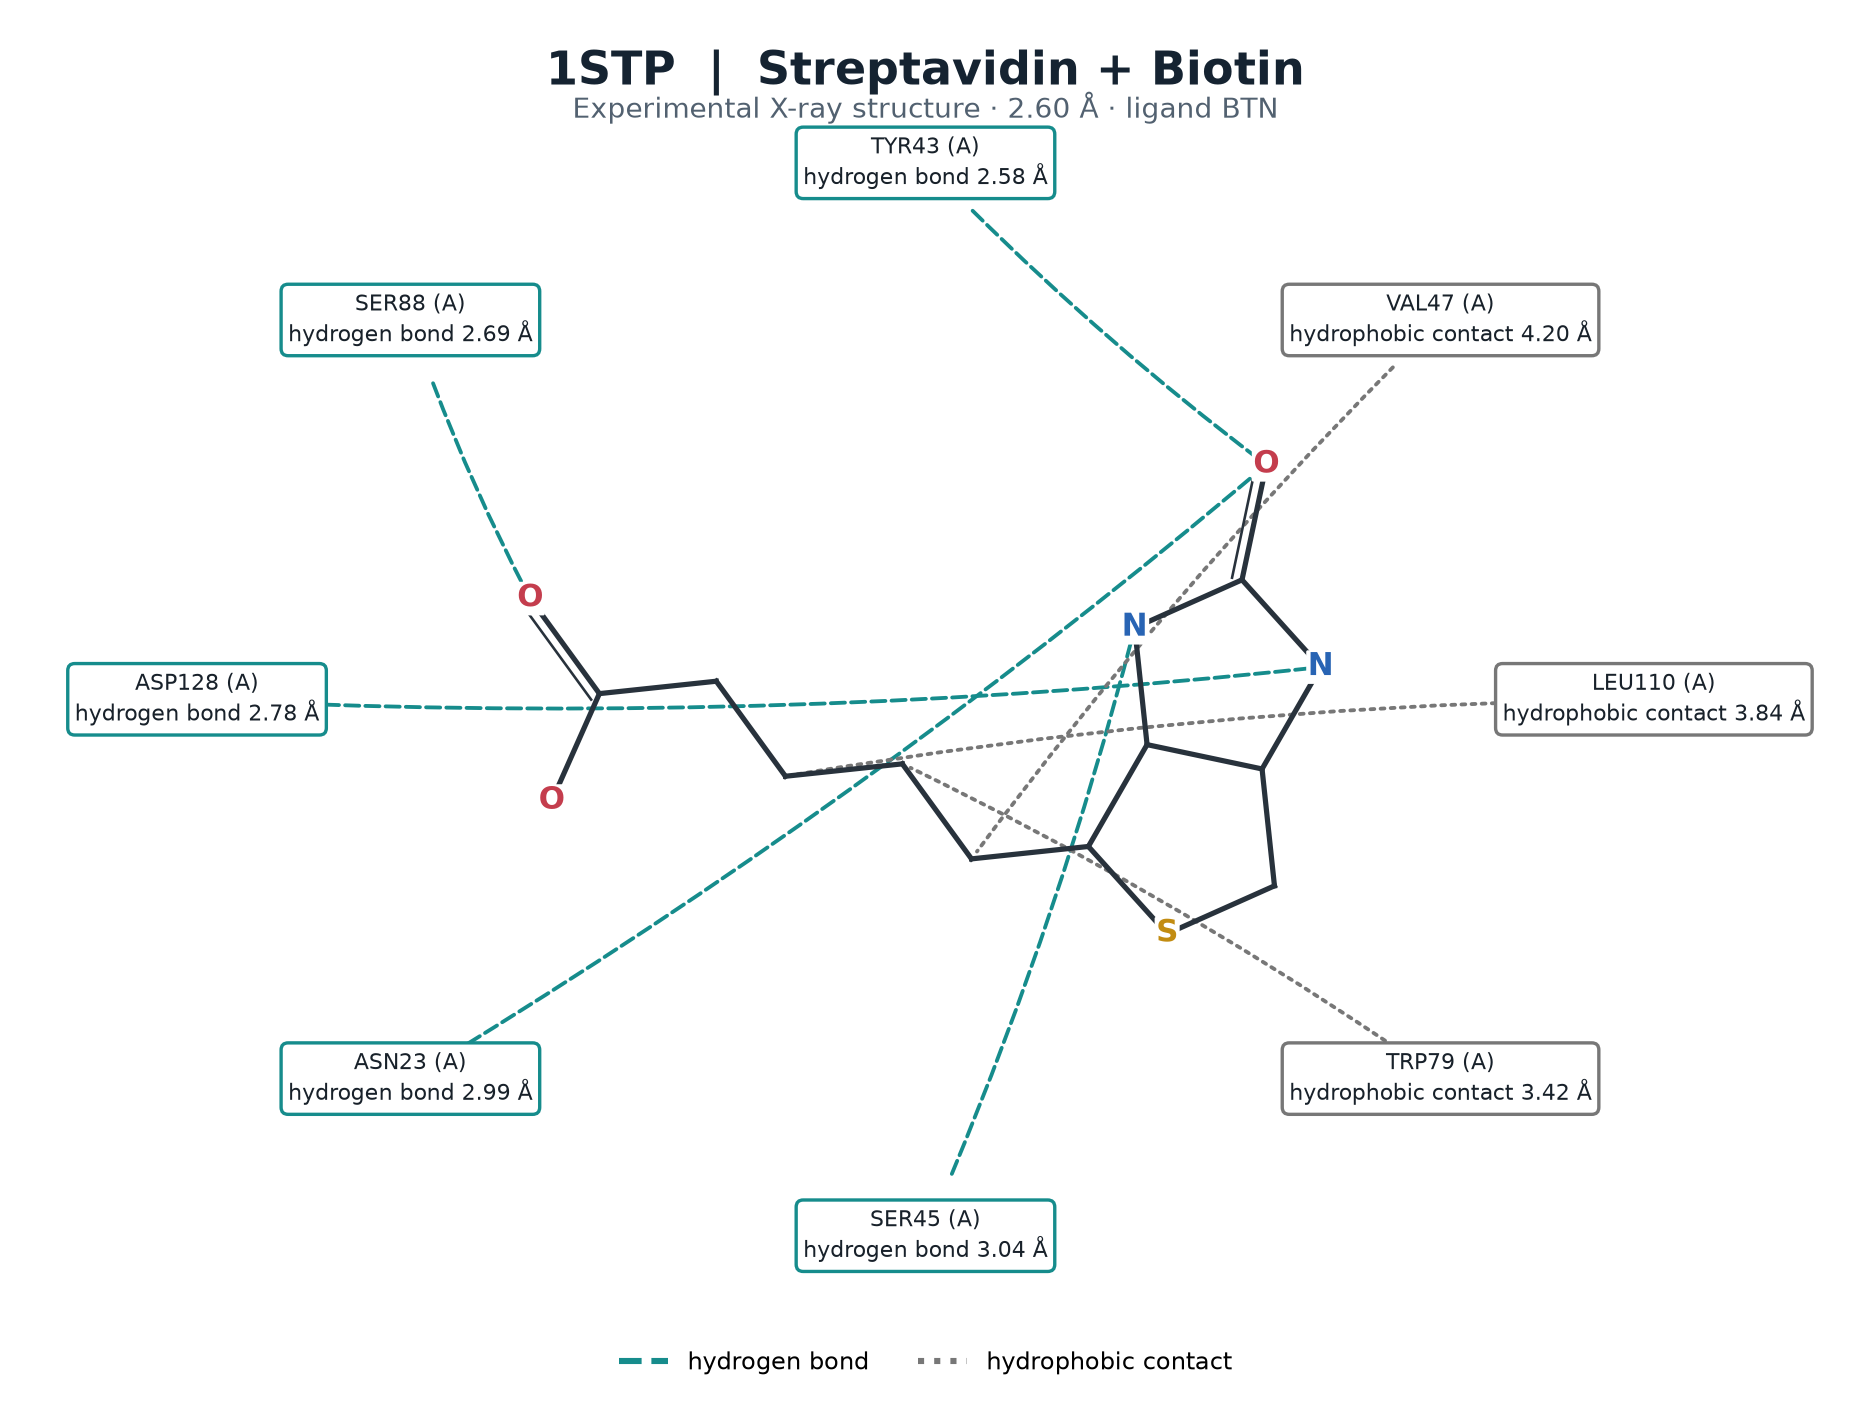
\includegraphics[width=\linewidth]{figures/interaction_1STP.png}\caption{1STP: streptavidin--biotin}\end{subfigure}\caption{Interaction diagrams generated from five separate experimental structure demonstrations.}\label{fig:structural}\end{figure}
